% This is "sig-alternate.tex" V1.9 April 2009
% This file should be compiled with V2.4 of "sig-alternate.cls" April 2009
%
% This example file demonstrates the use of the 'sig-alternate.cls'
% V2.4 LaTeX2e document class file. It is for those submitting
% articles to ACM Conference Proceedings WHO DO NOT WISH TO
% STRICTLY ADHERE TO THE SIGS (PUBS-BOARD-ENDORSED) STYLE.
% The 'sig-alternate.cls' file will produce a similar-looking,
% albeit, 'tighter' paper resulting in, invariably, fewer pages.
%
% ----------------------------------------------------------------------------------------------------------------
% This .tex file (and associated .cls V2.4) produces:
%       1) The Permission Statement
%       2) The Conference (location) Info information
%       3) The Copyright Line with ACM data
%       4) NO page numbers
%
% as against the acm_proc_article-sp.cls file which
% DOES NOT produce 1) thru' 3) above.
%
% Using 'sig-alternate.cls' you have control, however, from within
% the source .tex file, over both the CopyrightYear
% (defaulted to 200X) and the ACM Copyright Data
% (defaulted to X-XXXXX-XX-X/XX/XX).
% e.g.
% \CopyrightYear{2007} will cause 2007 to appear in the copyright line.
% \crdata{0-12345-67-8/90/12} will cause 0-12345-67-8/90/12 to appear in the copyright line.
%
% ---------------------------------------------------------------------------------------------------------------
% This .tex source is an example which *does* use
% the .bib file (from which the .bbl file % is produced).
% REMEMBER HOWEVER: After having produced the .bbl file,
% and prior to final submission, you *NEED* to 'insert'
% your .bbl file into your source .tex file so as to provide
% ONE 'self-contained' source file.
%
% ================= IF YOU HAVE QUESTIONS =======================
% Questions regarding the SIGS styles, SIGS policies and
% procedures, Conferences etc. should be sent to
% Adrienne Griscti (griscti@acm.org)
%
% Technical questions _only_ to
% Gerald Murray (murray@hq.acm.org)
% ===============================================================
%
% For tracking purposes - this is V1.9 - April 2009

\documentclass{sig-alternate}
\usepackage{graphicx}
\usepackage[table]{xcolor}
\usepackage[usenames,dvipsnames]{color}


\graphicspath{{img/}}

\begin{document}
%
% --- Author Metadata here ---
\conferenceinfo{IIWAS}{2010 Paris, France}
%\CopyrightYear{2007} % Allows default copyright year (20XX) to be over-ridden - IF NEED BE.
%\crdata{0-12345-67-8/90/01}  % Allows default copyright data (0-89791-88-6/97/05) to be over-ridden - IF NEED BE.
% --- End of Author Metadata ---

\title{{\ttlit Morpheus}: An Ontology-based Question Answering System}

%\titlenote{A full version of this paper is available as
%\textit{Author's Guide to Preparing ACM SIG Proceedings Using
%\LaTeX$2_\epsilon$\ and BibTeX} at
%\texttt{www.acm.org/eaddress.htm}}}
%
% You need the command \numberofauthors to handle the 'placement
% and alignment' of the authors beneath the title.
%
% For aesthetic reasons, we recommend 'three authors at a time'
% i.e. three 'name/affiliation blocks' be placed beneath the title.
%
% NOTE: You are NOT restricted in how many 'rows' of
% "name/affiliations" may appear. We just ask that you restrict
% the number of 'columns' to three.
%
% Because of the available 'opening page real-estate'
% we ask you to refrain from putting more than six authors
% (two rows with three columns) beneath the article title.
% More than six makes the first-page appear very cluttered indeed.
%
% Use the \alignauthor commands to handle the names
% and affiliations for an 'aesthetic maximum' of six authors.
% Add names, affiliations, addresses for
% the seventh etc. author(s) as the argument for the
% \additionalauthors command.
% These 'additional authors' will be output/set for you
% without further effort on your part as the last section in
% the body of your article BEFORE References or any Appendices.

\numberofauthors{1} 
\author{
	 \alignauthor Christan Grant, Clint P. George, Joir-dan Gumbs, Joseph N. Wilson, Peter J. Dobbins \\
	 \affaddr{University of Florida, Dept. of Computer Science} \\ \affaddr
{ Gainesville, Florida, USA} \\
\email{\{cgrant, cgeorge, jgumbs, jnw, pjd\} @cise.ufl.edu}
}

\date{2 July 2010}


\maketitle

% Abstract 
\begin{abstract}
- It is difficult to answer questions that change over time
- However, if the method of answering the question can be realized, the question can be easily answered
- We are building a system that supports a learning how to answer particular questions
- We can answer questions that are semantically similar to our store of questions
- We do this by building a semantic library ...
\end{abstract}


% A category with the (minimum) three required fields
%\category{H.4}{Information Systems Applications}{Miscellaneous}

% A category including the fourth, optional field follows...
%\category{D.2.8}{Software Engineering}{Metrics}[complexity measures, performance measures]

%\category{H.3.3}{Information Search and Retrieval}{Query formulation, Search process}
\category{H.3.4}{Systems and Software}{Question-answering (fact retrieval) systems}
%\category{I.2.6}{Learning}{Concept learning}[Parameter Learning]
%\category{I.2.7}{Natural Language Processing}{Language parsing and understanding, Text analysis}


% \terms{Experimentation, Theory}

\keywords{Deep web, ontology creation, NLP, semantic query matching, question answering}


% Introduction 
\section{Introduction}

% Outline 
% ---------------------

% 1. Motivation 
% 2. What are we proposing?  
% 3. Challenges
% 		3.1 User query processing 
% 		3.1 Need of an ontology 
% 4. Realm based question answering 
% 5. About the paper structure 

When traveling though a jungle to a destination, it is easy to get lost.  The first person to journey somewhere may make a number of mistakes when trying to find the best path to their destination. Those who come later find it easier to reach the destination if a well-marked trail has been created. Olsen and Malizia describe this idea as \emph{exploiting trails} \cite{5379671}.  Rather than treating a user's discovery experience as a unique entity, one can exploit the fact that a similar search may have already been performed.  In one study, almost 40 percent of all queries were repetitions of previous queries\cite{1277770}. Thus, reuse of prior searches is one way to optimize the search
process.  Morpheus is a question answering system motivated by reuse of prior web search pathways to yield an answer to a user query. Morpheus follows path-finders to their destinations and not only marks the trail, but also provides a taxi service to take followers to similar
destinations.

There are two distinct Morpheus user roles. A
\textit{path-finder} enters queries in the Morpheus web interface and
searches for an answer to the query using an instrumented web browser. 
This web tracking tool stores the query
and necessary information to revisit the pathways to the page where the path-finder 
found the answer. A \textit{path-follower} uses the Morpheus system much like a regular search engine with a natural language interface. The path-follower enters a question in a text box and receives a guided path to the answer. The system exploits previously found paths to provide an answer.

Morpheus represents user-query details in a semi-structured query (SSQ). It assumes the terms belong to classes of a \textit{consistent} realm-based ontology, that is, one having a singly rooted heterarchy whose subclass/superclass relations have meaningful semantic interpretations. When a path-follower enters a query, Morpheus ranks SSQs in the store based on class similarity. Suppose a regular user asks -\textit{ a 1997 Toyota Camry V6 needs what size tires?} In this query the classes associated with terms, e.g. \emph{Manufacturer} with \emph{Toyota}, helps us identify similar queries.


This paper discusses related question answering and ontology generation systems in section \ref{sec:relatedwork}. Section \ref{sec:systemarch} explains the Morpheus system and its implementation. In Section \ref{sec:results} we describe the current results of our approach.  Finally, we conclude with future goals for the system.


% Related Work 
\section{Related Work}
\label{sec:relatedwork}

\subsection{Question Ansering Systems} 

Question Answering (QA) is an old field and there has been a recent influx of QA work. The earliest question answering systems include BASEBALL \cite{Green1961} and Lunar \cite{woods1973} were both \emph{closed domain} and \emph{closed corpus}.  Closed domain QA systems are those in which the possible meanings of the questions given are finite. We define closed corpus sytems as those in which the sources used to answer questions are finite.  QA systems that treat the web as a document collection is considered an open corpus system.  The morpheus system is considered an open corpus system.  It goes beyond current state of the art QA systems by examining deep web sources.

Several community QA systems have been developed, one of the most popular being Yahoo! Answers \cite{yahooanswers2008}.  These sites enlist a community of users to answer question posed by other users.  This idea has evolved to invent socially integrated QA systems have emerged such as Aardvark \cite{vark2010}. In addition to having questions answered by users, aardvark is able to contact potential answers through several mediums beyond its webpage (e.g. instant message, mobile phone).  This allows for a possibly faster answers to questions.  The morpheus system relies on both user interface and the property of similar question being answered by a community of users to give a fast reliable answer.


\subsection{Ontology generators} 
\label{sec:ontology_generators}

An ontology formally models real world \textit{concepts} and their
relationships. A concept or class in an ontology gives us an abstract and
simplified view of the world\cite{Gruber1993} in a machine-readable and
language-independent format. The relationships and attributes of an
ontological concept are defined using \textit{properties} and \textit{property
restrictions}. An ontology definition contains all of
these: classes, properties, and restrictions. A class in an ontology can have
multiple \textit{super classes} and \textit{sub-classes}. Finally, a
\textit{knowledge base} represents an ontology together with 
instances of its classes.      

The DBpedia\footnote{http://dbpedia.org} project is based on extracting 
semantic information from the Wikipedia and making it available on the Web. 
Wikipedia semantics includes info-box templates, categorization information, 
images, Geo-coordinates, links to external Web pages, disambiguation pages, 
and redirects between pages in Wiki markup form \cite{Auer07dbpedia:a, Bizer2009}. 
DBpedia represents the Wikipedia categories using skos:concepts and category 
relations using skos:broader \cite{Auer07dbpedia:a, Bizer2009}. In fact, 
DBpedia does not define any new relations between the Wikipedia categories. 
The Wikipedia categories are extracted directly from Wikipedia pages, and there 
is no quality check on the resultant ontology. Similarly, additional ontological 
relations in DBpedia are generated from the info-box attributes and their values.

YAGO is a semi-automatically constructed ontology from Wikipedia and
WordNet\cite{Suchanek2009phd}. The YAGO ontology uses an automated process to
extract information from Wikipedia pages, info-boxes, and categories and to
combine this information with the WordNet\footnote{http://wordnet.princeton.edu}
synsets heterarchy. Since Wikipedia contains more individuals in the form of
Wikipedia pages than in the man-made WordNet ontology, the Wikipedia page titles
are used as the YAGO ontology individuals. YAGO concentrates mainly on the
fields of people, cities, events, and movies\cite{Suchanek2009phd}. 

In addition, YAGO uses Wikipedia categories as its ontology classes. The
ontology's heterarchy is built using the \textit{hypernym} and \textit{hyponym}
relations of the WordNet synsets. YAGO uses only the nouns from WordNet and
ignores the WordNet verbs and adjectives. The connection between a WordNet
synset and a Wikipedia category is achieved by parsing the category names and
matching the parsed category components with the WordNet
synsets\cite{Suchanek2009phd}. Those Wikipedia categories having no WordNet
match are ignored in the YAGO ontology.  
  
However, YAGO type extraction is mainly based on the assumption that
each Wikipedia page has at least one tagged category, and the assigned Wikipedia
categories are relevant to that Wikipedia page. The Wikipedia page category
assignments are subjectively assigned by human editors and some Wiki pages are
unassigned i.e., they have no category. In addition, we cannot completely rely
on the relevance of these assigned Wikipedia page categories. 


\subsection{NLP Interfaces} 


% System arch.
\section{System Architecure}
\label{sec:systemarch}

This section presents ontology and copora, query processing, ranking queries, and query executing.

\subsection{Using Ontology and Corpora} 
\label{sec:ontology_corpora}

Morpheus uses an ontology that contains categories of a particular realm of interest. Every leaf node in the ontology is associated with a corpus of words belonging to a category.  For example, we have constructed an automotive ontology containing categories relevant to the automotive realm. This ontology provides a structure for reference in the following sections.

Morpheus uses the DBpedia categories, Wikipedia pages and the WordNet synset heterarchy to construct ontologies. This approch is motivated by YAGO \cite{Suchanek2009phd}. First a realm is mapped to a DBpedia category \cite{Bizer2009}. 
Then a \emph{Markov Blanket} \cite{PRIS} is created covering all neighboring categories and using the DBpedia ontology properties \emph{broader} and \emph{narrower}. From here, the system recursively includes all categories up to the root.  

Once we have the categories belonging to a particular realm, we associate them with WordNet synsets using an approach similar to YAGO\cite{Suchanek2009phd}. We determine a \emph{head noun} in the category name and search for it in the WordNet synsets. DBpedia categories having no WordNet synset match are excluded from our ontology. 

To build a corpus for each of the leaf nodes in the ontology, 
we extract \emph{terms} from the Wikipedia pages associated with the 
the DBpedia categories. From this term corpus, 
we can find the likelihood of a term belonging to a particular category. This assists in categorizing terms in a \emph{path-follower} query.
The likelihood is determined by the probability of a category given a term 
using \textit{Bayes Rule} (Eq. \ref{eq:bayesrule}), since we can 
easily obtain the term-category and term-corpus probabilities as 
relative frequencies. 

\begin{equation}
\label{eq:bayesrule}
P (category | term) = \frac{P(term | category) P(category)}{P(term)}
\end{equation}    

In addition, we evaluate Latent Dirichlet Allocation (LDA) to identify latent topics of the documents in a corpus \cite{Blei2003latentdirichlet}.  LDA is Bayesian model represents a document in the corpus by distributions over topics, and a topic itself is a distribution over all  terms in the corpus.  For example, for the Wikipedia pages, the latent topics reflect the thematic structure of the pages. Thus, LDA can discover relevant topic proportions in a document using posterior inference \cite{Blei2003latentdirichlet}. Additionally, given a text document, using LDA we could tag related documents by matching the similarity over the estimated topic proportions, which is useful in the ontology and corpora building.  Due to its fully generative semantics, even at the level of documents, LDA could address the drawbacks (such as dimensionality and failure in finding the discriminative set of words for a document) of frequency based approaches such as TF-IDF, LSI, and pLSI.


\subsection{ Recording}
\label{sec:query_processing}
  
The \emph{Query Resolution Recorder} (QRR) is an instrumented web browser
used to track the search pathways to an answer for a \textit{path-finders} query. It
also helps guide to identify categories (optional) for the query terms. 
Morpheus has two types of categories: \emph{input categories} and \emph{output categories}.
Input categories annotates the query terms into a class or category, which are 
useful in finding similar queries. On the other hand, output categories give hints
to the expected answer of a user query. Morpheus captures all
this query information in the representation of an SSQ. For example, suppose, a guide 
tries to answer the query ``A 1997 Toyota Camry V6 needs what size tires?'', using
Morpheus. With the help of the QRR, guide may choose relevant query terms and assign
\emph{input categories} to them: Toyota : manufacturer, Camry V6 : 
model, tire : automotive parts, and size as the \emph{output category}. 
In addition, guide can log the search pathways to an answer (e.g. P215/60R16)
to this query and select the query \emph{realm} as automotive.      


The \emph{Query Resolution Method} (QRM) is a data structure that models the
question answering process. A QRM is usually constructed by a \emph{guide} with
the help of the QRR. Each QRM contains an \emph{ontological realm}, an SSQ, and
information to support the query answering process. QRMs are associated with an
ontology that has a particular realm i.e. an ontological realm. In addition, 
the QRM contains information required to visit each page needed to 
answer the query as well as the order of visitation. For each
dyanamic page, it stores the list of inputs to the URL such as form inputs and
the possible referrence outputs (highlighted portions of the web page).


% NLP arch. 
% Joir-dan

Rather than working blindly, forming all possible n-grams from the query 
and running probabilities, it seemed to be a better approach to identify 
important noun phrases within the query, and work with those. Using our 
query parser, we proceed to tokenize, parse, and chunk our candidate query, 
extracting verb groups, answer classes, and descriptive info from each query. 
In the example query "What is the tire size of a 1997 Toyota Camry?," 
the verb group is the verb "is," the answer class is "tire size," and descriptive 
info is "of a 1997 Toyota Camry." The next step is to create n-grams from these chunks. 
Using these n-grams, we will query our database for frequencies associated with 
each n-gram: overall frequency and categorical frequency, alongside category 
term count and overall term count, to calculate categorical probabilities 
and establish a realm for the candidate query, choosing realm with highest probability.




\subsection{Ranking} 
\label{sec:qrm_ranking}

To answer a user's query, a \textit{candidate
SSQ}, Morpheus finds similar SSQs that belong to QRMs in the Morpheus data store (a \textit{qualified SSQ}). We need a similarity measure to match the candidate SSQ
with a qualified SSQ. For the SSQ similarity, we
consider the SSQ components such as query-realm, input
terms and output terms, and their assigned categories or classes [To be changed]. The,
\textit{category divergence} of two categories characteristics their 
similarity based on an ontology class heterarchy. 
It is motivated by the concept of multiple
dispatch in CLOS and Dylan programming for generic function \emph{type} matches. 

We consider the category match as a type match and we use 
\emph{category divergence} to calculate the relevance between 
the candiate SSQ and a qualified SSQ. Each qualified SSQ will 
have input terms, output terms, and associated classes, and one realm (from QRM). 
For the candidate SSQ, the relevant categories for terms 
are determined from the NLP engine and corpora. The calculation of a realm 
for a candidate query is done using the n-grams found within said query 
and the probabilities (if any) found using frequencies within the database.
We match QRMs that belong to the same \emph{realm} of the candidate SSQ. 
The relevance of a qualified SSQ to the candidate SSQ is 
determined by aggregating the divergence measure of input-term-categories 
associated with them. In addition, we order QRMs in the data store 
by descreasing relevance. The order provides a ranking for the results 
to the user. The following subsection describes \emph{category divergence} 
in detail.

\subsubsection{Catgeory Divergence}
\label{sec:ctd}

We employ a quasimetric, \textit{category
divergence (cd)},
between a source category and a target category using the \textit{topological
structure} of the categories in an ontology. We write $S \prec T$ for the
reflexive
transitive closure of the supercategory relation. Let $d(P,Q)$ represent the hop
distance in the directed ontology inheritance graph from $P$ to $Q$. The
divergence between a source and target category ranges from zero (for identical
categories) to one (for type incompatible categories). Let $S$ be the source
category, $T$ be
the target category, and $C$ be a least common ancestor category of $S$ and
$T$ i.e., one that minimizes $d(S,C) + d(T,C)$. The category divergence between $S$ and $T$ is defined given by:

\begin{equation}
cd(S, T) = \begin{cases}
0 & S.{Uri} \equiv T.{Uri}\\
d(S, T)/(3h) & S \prec T\\
1 & T \prec S\\
(d(S,root) + d(S,C) \\ \ \ \ \ + d(T,C))/(3h) & otherwise
\end{cases}
\end{equation}

\noindent where $h$ is the height of the ontology tree.

Note, if $S \prec T$ and $S \not\prec Q$ then $cd(S,T) <
cd(S,Q)$, that is, the divergence of a source category to a target
ancestor category is smaller than the divergence of a source category to any
category that is not an ancestor. This is an important property in
determining the compatibility of categories for answering queries.  If a
SSQ answers queries concerning an ancestor category, it is more relevant
that a SSQ that answers queries from any non-ancestral category.

% Algorithm 1: figure  
\begin{figure}[t]
\centering
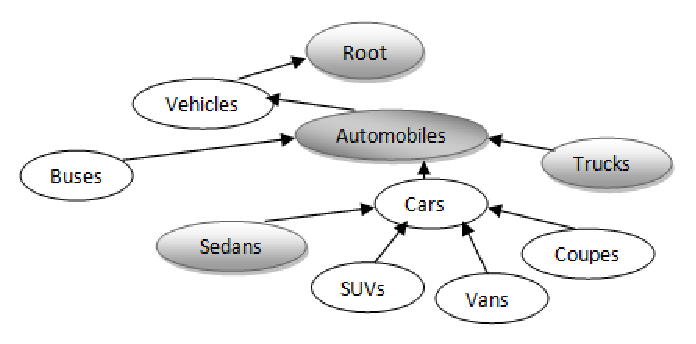
\includegraphics[width=85mm]{img/automotive_ontology.eps}
\caption{An abbreviated man-made automotive ontology - arrows represent inheritance relationships between the ontological classes.}
\label{fig:automotive_ontology}
\end{figure}

Suppose we want to find the category divergence between \textit{Sedans}
and \textit{Trucks} (Figure \ref{fig:automotive_ontology}). 
\textit{Sedans} is the subcategory of \textit{Cars}, and \textit{Trucks}
is the subcategory of \textit{Automobiles}. Therefore, the least common ancestor ($C$)
for these twoThis section presents ontology and copora, Query processing, ranking queries, and the query resolution mechanism. categories is \textit{Automobiles}. In addition, the tree height \textit{h = 4}.
So, the normalized divergence $cd$\textit{(Sedans, Trucks)} is \textit{7/12}
that is calculated from \textit{d(Sedans, Root) = 4}, \textit{d(Sedans, Automobiles) = 2}, and \textit{d(Trucks, Automobiles) = 1}.


\subsection{Executing} 

QRM contains the necessary  
information required to re-run this procedure.Once we have 
relevant QRMs through QRM ranking for a given user query, we can  
get answers by re-running the pathways with help of 
the \emph{Query Resolution Engine} (QRE) of Morpheus. 



% Results and conclusion  
\section{Results}
\label{sec:results}

% 3-4 queries 
% Human made ontology 
% Topic Models 

As an initial step we created a man-made realm-ontology for the automotive realm
 exploiting the Wikipedia pages, categories, and WordNet synsets. For each of
the categories in the realm-ontolgy we built corpora by grabbing the
corresponding Wikipedia pages. The following section describes question
answering process for a user query, ``A 1997 Toyota Camry V6 needs what size
tires?''

The Morpheus NLP engine parses this query into the constructs: WH:what,
Descriptive Information:1997 Toyota Camry V6, Asking For:size tires. From the
descriptive info, we generate the N-grams or terms 1997, 1997 Toyota, 1997
Toyota Camry,Toyota,Toyota Camry,Toyota Camry V6, Camry, Camry V6, and V6. For
each of the terms, we determined relevant categories (non-increasing order of
relevance) from the ontology corpora. Table \ref{tbl:term_categories} shows
the top categories and their probabilities for each of the query term: 

\begin{table}[h]\footnotesize

\begin{tabular}{l | l | r}
Term & Category & $P(Category|Term)$ \\
\hline
1997 & Sedans & 404132.77e-14\\
1997 Toyota & Engines & 7.90e-14\\
Toyota  & Sedans & 3486670.15e-14\\
Toyota Camry & Sedans & 12147.23e-14\\
Toyota Camry V6 & Coupes & 13.80e-14\\
Camry & Sedans & 312034.20e-14\\
Camry V6 & Coupes & 13.80e-14\\
V6 & Sedans & 4464535.40e-14\\
\hline
\end{tabular}        

\caption{Terms' top categories and probabilities}
\label{tbl:term_categories}   

\end{table}

We used this top category of each of the terms in the candidate SSQ and
determined the category divergence with the qualified SSQ categories in the QRM
store. We assumed that all of them belong to the same realm or domain (but, it
is different in real time). In the end, we combined the divergence measure and
ranked QRMs based on the relevance score. Table \ref{tbl:ranked_queries}
shows the top ranked queries that belong to the QRMs in store for the above
query.

\begin{table}[h]\footnotesize

\begin{tabular}{l | r}
Query & Score\\
\hline
A 1997 Toyota Camry V6 needs what size tires? & 0.91\\ 
What is the tire size for a 1998 Sienna XLE Van? & 0.72\\ 
What is the tire size for a 1996 Infiniti I30 Sedan? & 0.88\\ 
\hline
\end{tabular}        

\caption{Top ranked queries and relevance scores}
\label{tbl:ranked_queries}   

\end{table}


%\subsection{Discussion}
\section{Conclusion}

In this paper, we proposed a novel question answering method based on a realm-based ontology. [How do we calculate relam for a candidate query? and NLP]. This query matching strategy assumes that candidate query terms are available in the category corpus. The candidate query's category annotation will fail if the
query terms are not available in the corpus. In addition, classification of a term or n-gram into a category is based on the term frequency distributions in a classified web document. We are working on improving this
approach by using a probabilistic generative approach as used in the Topic
Models\cite{Blei2003latentdirichlet}. 

Similarly, the Morpheus ontology building
process needs categorized web pages. As explained in section
\ref{sec:ontology_generators}, the Wikipedia page categories have some
limitations for this purpose. Without supervision, the page categorization is
often a challenging problem, because topics in the pages that belong to a realm
(e.g. automotive) usually overlap. So we are evaluating the applicability of
probabilistic topic models to web page categorization, and automatic
generation of a realm-ontology based on the topics being extracted.            
 


% 2. Current stage of the project 
% 3. Expected contribution to the topics of interest supported by iiWAS2010 




\section{Acknowledgments}

Our thanks to Ben Landers, Patrick Meyer, and Terence Tai for their assistance building this system. Additionally, we would like to thank NSF for their generous support of our project.

% Bibliography 
\bibliographystyle{abbrv}
\bibliography{morpheus}  


\end{document}
